\section{Diseño}

\subsection{planteamiento de circuito}
Como se mencionó anteriormente, utilizando el módulo de matriz de leds MD\_7219.
Utilizando el microcontrolador Arduino Uno, utilizando las entradas digitales se debe 
colocar que lean los botones, siendo este uno rojo y azul. El botón rojo debe hacer que la matriz 
incremente en uno el contador que se lleva hasta llegar a F, si se pasa de F este debe volver a 0. El botón
azul debe hacer que la cuenta disminuya por cada toque hasta llegar a 0, si este se presiona nuevamente se debe
regresar a F. Teniendo el anterior planteamiento y conectando el módulo directo a la placa, con la alimentación
de $\SI{5}{\volt}$ y a tierra, se tiene el siguiente diagrama:
\begin{figure}[h!]
    \centering
    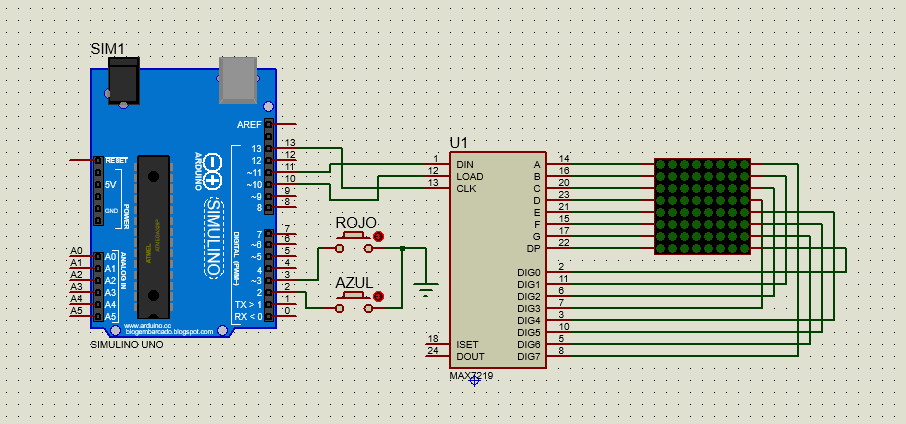
\includegraphics[width=0.8\textwidth]{Diagramas/Diagrama.png}
    \caption{Diagrama de conexión}
    \label{fig:conexion}
\end{figure}

Ahora bien, ya que el módulo no existe en el simulador, se construyó utilizando el circuito integrado y una matriz de LEDs entregadas por el programa. Igualmente, se observan ambos botones conectados a tierra. Estos botones están en configuración de pull up, es decir que los pines están energizados en $\SI{5}{\volt}$ mediante una resistencia de pull up, entregando el valor HIGH,
si se presiona el botón, este pasa a LOW, teniendo así las entradas digitales de nuestro montaje. Para la salida de nuestro circuito 
se tiene la matriz construida, así esta se tiene que conectar a un voltaje de alimentación y a tierra, pero en Protheus no se puede realizar esto, 
pero teniendo considerado esto para la implementación del circuito.

\subsection{Desarrollo del código}
Para el desarrollo del código que se implementa en el Arduino Uno, se utilizó la biblioteca \texttt{MD\_MAX72xx}, se usó
el recurso \cite{programarfacilMax7219} para aprender de los comandos de la biblioteca. Y la biblioteca \texttt{SPI} para 
la comunicación entre el módulo y el Arduino Uno. Así el código hecho se observa en \autoref{lst:cod-1}. A continuación, se explicará 
bloque a bloque la lógica de este.
\clearpage
\begin{listing}[H]
    \begin{minted}{cpp}
        #include <MD_MAX72xx.h>
        #include <SPI.h>

        #define hardware MD_MAX72XX::GENERIC_HW
        #define pinDIN 11
        #define pinCS 10
        #define pinCLK 13

        MD_MAX72XX mx = MD_MAX72XX(hardware,pinDIN,pinCLK,pinCS,1);

        const int botonPin1 = 3;  
        const int botonPin2 = 2;
        int contador = 0;         
        int estadoAnterior = HIGH; 
        int estadoAnterior2 = HIGH;
    \end{minted}
    \caption{Definición de variables}
    \label{lst:b1}
\end{listing}

Como se mencionó anteriormente, las bibliotecas utilizadas sirven para comunicarse y controlar el módulo. Ahora bien en \autoref{lst:b1},
primero se definieron los pines y el hardware utilizado en este caso, siendo el genérico, para luego definir un objeto
\texttt{mx} con las especificaciones definidas en las líneas anteriores.   

\begin{listing}[H]
    \begin{minted}{cpp}
        void setup() {
            mx.begin();

            mx.setChar(5,'0');
            pinMode(botonPin1, INPUT_PULLUP); 
            pinMode(botonPin2, INPUT_PULLUP);
            Serial.begin(9600);
        }
    \end{minted}
    \caption{Setup del código}
    \label{lst:b2}
\end{listing}
En \autoref{lst:b2}, se inicia la matriz de leds y los pines definidos en \autoref{lst:b1}, cabe destacar que en el diseño se consideraron estos botones
de Pull up, para esto se tendría que colocar una resistencia, pero el Arduino Uno posee esta resistencia en el pin, utilizando \texttt{INPUT\_PULLUP} esta se activa.
Una vez iniciado el circuito este mostrará siempre el cero al iniciocomo se observa en el bloque. Por último, se inicia la comunicación
serial a $\SI{9600}{\frac{\bit}{\second}}$.

\clearpage
Para la parte de \texttt{loop()}, se separar en dos partes la explicación de este, una parte para el botón rojo y otro para el botón azul. Para el primer botón, se tiene:

\begin{minted}{cpp}
        int estadoActual = digitalRead(botonPin1);
        if (estadoAnterior == HIGH && estadoActual == LOW) {
            mx.clear();
            contador++;
            if(contador>15) contador = 0;
            if (contador <= 9){
                mx.setChar(5,'0'+contador);
            }
            else if (contador>=10 && contador<=15){
            mx.setChar(5,'7'+ contador);
            }
    
            Serial.println(contador);
            delay(200); 
        }
        estadoAnterior = estadoActual; 
    \end{minted}

\subsection*{Botón de incremento (Botón 1)}
El código implementa un control de estado para el botón, (antirrebote). Lo cual es importante para asegurar que cada pulsación del botón se interprete de forma correcta.

La lógica es la siguiente:
\begin{itemize}
    \item La línea \texttt{1} lee el estado actual del botón y lo almacena en la variable \texttt{estadoActual}.
    \item La condición \texttt{if (estadoAnterior == HIGH \&\& estadoActual == LOW)} en la línea \texttt{2} detecta un flanco de bajada, que corresponde al momento exacto en que el botón es presionado. Esta condición se cumple solo una vez por cada pulsación, garantizando un solo incremento.
    \item La línea \texttt{4} incrementa el contador.
    \item Las líneas \texttt{5--11} gestionan la lógica del contador para que opere en base 16 (hexadecimal). Si el valor del contador supera los \texttt{15}, la línea \texttt{5} lo reinicia a \texttt{0}.
\end{itemize}

La lógica para el botón de decremento es análoga a la del botón de incremento. Utiliza el mismo método de antirrebote para detectar el flanco de bajada.
\clearpage
\begin{listing}[H]
    \begin{minted}{cpp}
  int estadoActual2 = digitalRead(botonPin2);
 
  if (estadoAnterior2 == HIGH && estadoActual2 == LOW) {
    mx.clear();
    contador--;
    if(contador<0) contador = 15;
    if (contador > 9){
        mx.setChar(5,'7'+contador);
    }
    else if (contador<=9 && contador>=0){
      mx.setChar(5,'0'+ contador);
    }
    Serial.println(contador);
    delay(200); 
  }
    \end{minted}
\end{listing}

\subsection*{Funciones de la librería \texttt{MD\_MAX72XX}}

La librería MD\_MAX72XX hace mucho más sencilla la comunicación con el módulo y el control de la matriz de LEDs.

En este proyecto se utilizan principalmente dos funciones clave:
\begin{itemize}
    \item \texttt{mx.clear()}: Su tarea es "borrar la pizarra". Esta función apaga todos los LEDs de la matriz, asegurando que el nuevo valor se muestre de forma limpia, sin que quede rastro del número anterior.
    \item \texttt{mx.setChar(posicion, caracter)}: Esta función es la encargada de mostrar un carácter en un lugar específico de la matriz. Recibe dos parámetros:
    \begin{itemize}
        \item \texttt{posicion}: Indica la columna de la matriz donde aparecerá el carácter. En este caso, se usa el valor 5, que corresponde a una ubicación concreta de la pantalla.
        \item \texttt{caracter}: Es el símbolo que queremos mostrar. Como el contador trabaja en hexadecimal (de 0 a F), se hace una pequeña conversión matemática para pasar del valor numérico (0 a 15) al carácter correspondiente (0 a 9 y A a F). Para esto, se aprovecha el código ASCII: al sumar el valor del contador a la base '0' o '7', se obtiene automáticamente la letra o número correcto que debe verse en la matriz.
    \end{itemize}
\end{itemize}
